\chapter{KNN}

\section{Introduzione}
Si possono considerare gli esempi come punti in uno spazio $n$ dimensionale dove $n$ \`e il numero di features.
Per classificare un esempio $d$ si pu\`o mettere a $d$ una label uguale a quella dell'esempio pi\`u vicino a $d$ nel training set.
Questo concetto viene esteso nel $K$-nearest neighbour o \emph{K-NN} in cui per classificare un esempio $d$ si trovano i $k$ esempi pi\`u vicini di $d$ e si sceglie la label in maggior numero tra i $k$ vicini pi\`u prossimi. 
$k$ è l'unico iperparametro di \emph{K-NN}.
\emph{K-NN} \`e un modello non parametrico.

\section{Misurare la distanza}
Misurare la distanza (o similarit\`a) tra due esempi \`e specifico al problema, ma un modo possibile \`e la distanza Euclidea:
$$D(a,b)=\sqrt{(a_1-b_1)^2+\cdots+(a_n-b_n)^2}$$
Non ha sempre senso utilizzare la distanza Euclidea, nel caso in cui le feature non siano compatibili possiamo standardizzarle dividendole per la deviazione standard corrispondente. In questo modo tutte hanno la stessa importanza. Un'alternativa \`e utilizzare min-max scaling. 
Potremmo voler assegnare a feature un importanza differente, nel modello che classifica mele e arance la feature colore \`e più rilevante di quella del peso. 

In alternativa si pu\`o usare la distanza di Minkowski, che \`e una generalizzazione della distanza Euclidea:
$$D(a,b) = \sqrt[r]{\sum_{k=1}^{p}{|a_k - b_k|^r}}$$

\begin{multicols}{2}
	\begin{itemize}
		\item $r$ \`e un parametro, $p$ \`e il numero di dimensioni
		\item $r=1$ \`e la distanza Manhattan
		\item $r=2$ \`e la distanza Euclidea
		\item $r\rightarrow\infty$ \`e la distanza \textit{supremum}
	\end{itemize}
\end{multicols}

\begin{figure}
	\centering
	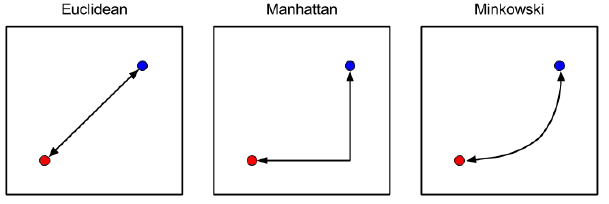
\includegraphics[width=0.6\linewidth]{imgs/chapter3/img2}
	\caption{Confronto tra le distanze}
	\label{fig:chapter03-02}
\end{figure}

	\subsection{Coseno di similitudine}
	
	Dati due vettori di attributi numerici, $d1$ e $d2$, il livello di similarità tra di loro \`e espresso utilizzando la formula:
	$$cos(d1,d2)=\frac{d1 \cdot d2}{||d1|| ||d2||}$$
	
	Dove con $\cdot$ indichiamo il prodotto scalare tra i due vettori e con $||d1||$ indichiamo la lunghezza del vettore. 
	Utilizzata spesso per confrontare blocchi di testo come documenti.

	\subsection{Distanza e similarit\`a}
	La misurazione della distanza/similarità \`e un problema specifico del dominio e ci sono molte, molte varianti diverse.
	\begin{itemize}
		\item Distanza: Misura numerica della differenza tra due oggetti di dati. Più bassa quando gli oggetti sono più simili tra loro. Il minimo di solito \`e 0, il massimo dipende dal problema.
		\item Similitudine: Misura numerica della somiglianza tra due oggetti di dati. È più alta quando gli oggetti sono più simili. Spesso rientra nell'intervallo [0,1].
	\end{itemize}
\section{Decision boundaries}
I decision boundaries sono posti nello spazio delle features dove la classificazione di un punto o un esempio cambia.
In particolare \emph{K-NN} definisce dei decision boundaries localmente tra le classi. 
La scelta di $K$ influenza la forma dei decision boundaries.

\section{Il ruolo di $K$}
I fattori che determinano la bont\`a di un algoritmo di machine learning sono la sua abilit\`a di minimizzare il training error e minimizzare il gap tra il training error e il test error.
Questi due fattori corrispondono a underfitting e overfitting \ref{fig:chapter03-00}.

	\subsection{Underfitting}
	L'underfitting avviene quando il modello non \`e capace di ottenere un valore di errore abbastanza piccolo sul training set.
	
	\subsection{Overfitting}
	L'overfitting avviene quando il gap tra il training error e il test error \`e troppo grande.
	
	\begin{figure}
		\centering
		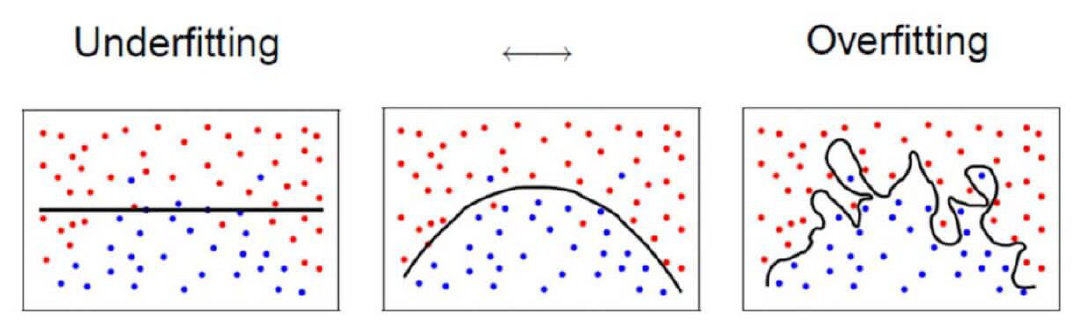
\includegraphics[width=0.6\linewidth]{imgs/chapter3/img1}
		\caption{Recap su overfitting e underfitting}
		\label{fig:chapter03-00}
	\end{figure}

\section{Scelta di $K$}
Il valore di $K$ comprende euristiche comuni come $3, 5, 7$ o un numero dispari per evitare pareggi. Tipicamente meno di $\sqrt{\mathcal{N}}$.
Pu\`o essere scelto utilizzando dati di sviluppo.
Per classificare un esempio $d$ si trovano i $k$ vicini pi\`u prossimi di $d$ e si sceglie la classe pi\`u presente nei $k$ scelti.

\begin{figure}
	\centering
	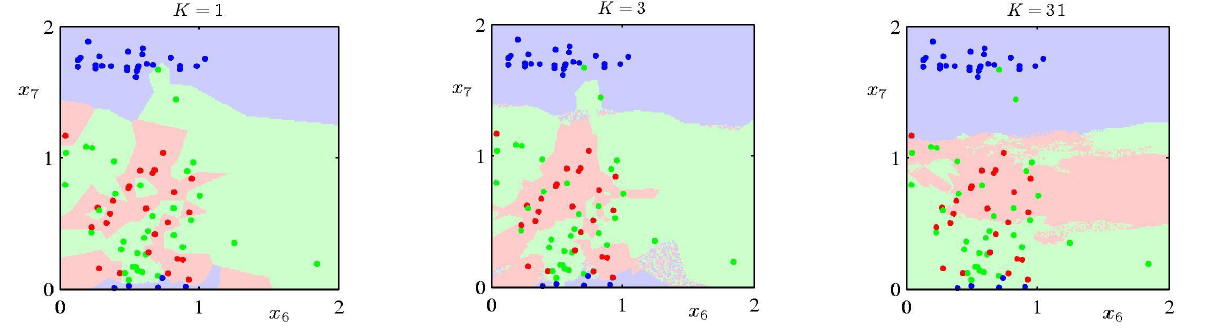
\includegraphics[width=0.6\linewidth]{imgs/chapter3/img0}
	\caption{L'impatto di $K$}
	\label{fig:chapter03-01}
\end{figure}

\section{Variazioni di $K$}
Invece di scegliere i $K$ vicini pi\`u prossimi si possono contare tutti gli esempi in una distanza fissata.

	\subsection{\emph{K-NN} pesata}
	Si pu\`o pesare il voto di tutti gli esempi in modo che esempi pi\`u vicini pesino di pi\`u.
	Si usa spesso qualche tipo di decadimento esponenziale.

\section{Lazy Learners vs Eager Learner}
\emph{K-NN} appartiene alla classe degli algoritmi detti \emph{lazy learner}.
Gli algoritmi \emph{lazy learner} sono algoritmi che memorizzano semplicemente i dati di training (o esegue un'elaborazione limitata) e effettua il calcolo solamente quando viene fornito un esempio di prova. 
Tipicamente impiegano meno tempo in fase di training rispetto agli algoritmi \emph{eager learner}, ma impiegano più tempo in fase di previsione. 
In \emph{K-NN} non c'\`e fase di training.
Gli algoritmi \emph{eager learner} (es: Decision Trees e SVMs) sono algoritmi che dato un insieme di training costruiscono un modello di classificazione prima di ricevere nuovi dati da classificare.


\section{Curse of dimensionality}

Il successo di \emph{K-NN} dipende molto dall'avere a disposizione un insieme di dati denso. 
Ogni algoritmo di apprendimento automatico ha bisogno di un insieme di dati denso per una previsione accurata. 
Ci\`o che rende \emph{K-NN} speciale è il fatto di richiedere che ogni punto sia vicino in ogni dimensione, altri algoritmi operano su una singola dimensione e necessitano che i punti siano vicini solo su quella.
All'aumentare del numero di dimensioni, anche la densit\`a dei dati da mantenere aumenta, senza un aumento delle dimensioni del dataset \emph{K-NN} perde potenza predittiva.


\section{Vantaggi e problemi di \emph{K-NN}}
	
	\subsection{Vantaggi}
	\begin{multicols}{2}
		\begin{itemize}
			\item Facili da programmare
			\item Non \`e necessaria alcuna computazione o training
			\item L'accuratezza della classificazione può essere molto buona, può superare modelli più complessi
		\end{itemize}
	\end{multicols}

	\subsection{Problemi}
	\begin{multicols}{2}
		\begin{itemize}
			\item La scelta della "distanza", tipicamente Euclidea
			\item Scelta di $K$
			\item Curse of dimensionality
			\item Ogni volta che vogliamo classificare un nuovo punto si deve fare una nuova scansione dell'intero dataset, proibitivo per dataset grandi.
		\end{itemize}
	\end{multicols}